\documentclass[12pt,a4paper]{article}
\usepackage{fullpage}
\usepackage{tensormatrix}
\usepackage{subfig}

\newlength{\pwidth}
\setlength{\pwidth}{8cm}

\begin{document}
\title{tensormatrix -- version 1.0.0}
\author{Einar Halvorsen}
\date{August 8, 2025}
\maketitle


This package helps visualizing the structure of matrices representing the tensors of linear constitutive equations. It requires the tikz package. The package provides an environment \textit{tmat} which takes two parameters, the dimensions of the matrix. The environment requires math mode. Inside the environment a sequence of commands can be given. The available commands are listed in table \ref{tab:elements}. They either define a symbol to appear at the location specified by the parameter of the command or a link between two elements. If no symbol is defined for an element, the default, a small dot, is shown. This would define a zero value in the usual use of the notation.   

\begin{table}[hbt]
  \centering
  \caption{Elements available, notation and usual interpretation}
  \label{tab:elements}
  \begin{tabular}{cll}
    \hline\hline
    Symbol & Command & Interpretation \\
    \hline
\begin{tikzpicture}
\node [tkz] (0,0) {};
\end{tikzpicture}
&  & a component that is zero
\\
\begin{tikzpicture}
\tmatpv{0}{0}
\end{tikzpicture}
& \verb|\tmatpv{M}{N}|  & element (M,N) that is nonzero
\\
\begin{tikzpicture}
\tmatpn{0}{0}
\end{tikzpicture}
& \verb|\tmatpn{M}{N}|&
\parbox[t]{\pwidth}{
element (M,N) has sign opposite to the one it is connected to}
\\
\begin{tikzpicture}
\tmatpdv{0}{0}
\end{tikzpicture}
&\verb|\tmatpdv{M}{N}| &
\parbox[t]{\pwidth}{
element (M,N) has twice the value of the solid-circle component it is connected to}
\\
\begin{tikzpicture}
\tmatpdn{0}{0}
\end{tikzpicture}
& \verb|\tmatpdn{M}{N}| &
\parbox[t]{\pwidth}{
  element (M,N) has minus twice the value of the solid-circle component it is connected to}
\\
\begin{tikzpicture}
\tmatpx{0}{0}
\end{tikzpicture}
& \verb|\tmatpx{M}{N}| &
\parbox[t]{\pwidth}{
element (M,N) is given by other elements}
\\  
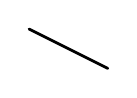
\begin{tikzpicture}
\draw[line width=1pt,line cap=round,fill=black] (-0.5\tmatds,.5\tmatds) -- (0.5\tmatds,0);
\end{tikzpicture}
& \verb|\tmatlink{M N}{P Q}| &
\parbox[t]{\pwidth}{connection between  elements (M,N) and (P,Q) with related values}
\\ \vspace{-1.5ex}\\  \hline
  \end{tabular}
\end{table}

Examples of typical use are provided by the matrices given in figure \ref{fig:matex}. 

\begin{figure}[h]
  \centering
  \subfloat[]{
    \label{fig:matexa}
  $\begin{tmat}{6}{6}
    \tmatpv{1}{1}
    \tmatpv{1}{2}
    \tmatpv{1}{3}
    \tmatpv{1}{4}
    \tmatpv{2}{1}
    \tmatpv{2}{2}
    \tmatpv{2}{3}
    \tmatpn{2}{4}
    \tmatpv{3}{1}
    \tmatpv{3}{2}
    \tmatpv{3}{3}
    \tmatpv{4}{1}
    \tmatpn{4}{2}
    \tmatpv{4}{4}
    \tmatpv{5}{5}
    \tmatpx{6}{6}
    \tmatpdv{6}{5}
    \tmatpdv{5}{6}
    \tmatlink{1 1}{2 2}
    \tmatlink{1 3}{2 3}
    \tmatlink{1 4}{2 4}
    \tmatlink{2 4}{5 6}
    \tmatlink{3 1}{3 2}
    \tmatlink{4 1}{4 2}
    \tmatlink{4 2}{6 5}
    \tmatlink{4 4}{5 5}
  \end{tmat}$
  }
  \hspace{2cm}
  \subfloat[]{
    $\begin{tmat}{3}{3}
      \tmatpv{1}{1}
      \tmatpv{2}{2}
      \tmatpv{3}{3}
      \tmatlink{1 1}{2 2}
    \end{tmat}$ 
  }
  \hspace{2cm}
  \subfloat[]{
    $\begin{tmat}{3}{6}
      \tmatpv{1}{1}
      \tmatpn{1}{2}
      \tmatpv{1}{4}
      \tmatpn{2}{5}
      \tmatpdn{2}{6}
      \tmatlink{1 1}{1 2}
      \tmatlink{1 2}{2 6}
      \tmatlink{1 4}{2 5}
    \end{tmat}$
  }
  \caption{Matrices for a material of with class-32 symmetry. (a) $S^E$, $S^D$. (b) $\kappa^\epsilon$, $\kappa^\sigma$, $\beta^\epsilon$, $\beta^\sigma$. (c) $d$.}
\label{fig:matex}
\end{figure}

\newpage
As an example of use, the code producing the matrix in figure \ref{fig:matexa} 
is:
\begin{verbatim}
\begin{tmat}{6}{6}
    \tmatpv{1}{1}
    \tmatpv{1}{2}
    \tmatpv{1}{3}
    \tmatpv{1}{4}
    \tmatpv{2}{1}
    \tmatpv{2}{2}
    \tmatpv{2}{3}
    \tmatpn{2}{4}
    \tmatpv{3}{1}
    \tmatpv{3}{2}
    \tmatpv{3}{3}
    \tmatpv{4}{1}
    \tmatpn{4}{2}
    \tmatpv{4}{4}
    \tmatpv{5}{5}
    \tmatpx{6}{6}
    \tmatpdv{6}{5}
    \tmatpdv{5}{6}
    \tmatlink{1 1}{2 2}
    \tmatlink{1 3}{2 3}
    \tmatlink{1 4}{2 4}
    \tmatlink{2 4}{5 6}
    \tmatlink{3 1}{3 2}
    \tmatlink{4 1}{4 2}
    \tmatlink{4 2}{6 5}
    \tmatlink{4 4}{5 5}
  \end{tmat}
\end{verbatim}


\end{document}
